%% =====================================================================
\section{The Value of Each Action}\label{sec:structure}
%% =====================================================================
Any reasonable policy must compare, in each slot, how much each action is expected to lower the AoII with how much energy it costs. This section derives the first quantity in closed form and shows what it implies for the decision. Throughout, we fix slot $t$, let $\xh=\hat X(t)$, and write
\begin{equation}\label{eq:rw}
r=p_{\xh},\qquad w=p_{1-\xh}.
\end{equation}
In words, $r$ is the probability that the state leaves the value the GS currently reports, and $w$ is the probability that it leaves the other value. By~\eqref{eq:source}, both are below $\frac12$.

\subsection{One-Step Expected AoII}
We first compute the expected AoII in slot $t+1$ for a given hypothesis $\Delta(t)=\delta$ and a given new status $\xh'=\hat X(t+1)$. By~\eqref{eq:aoii}, $\Delta(t+1)$ is either $\delta+1$ or $0$, so its expectation is $\delta+1$ times the probability in~\eqref{eq:pred}: $(\delta+1)p_{x_\delta}$ if the new status equals $x_\delta$, and $(\delta+1)(1-p_{x_\delta})$ otherwise. The three actions differ only in which status $\xh'$ they produce, and with what probability. We evaluate this expectation for each of them, assuming the packet is delivered, and average it over $\pi_t$.

\emph{Silence.} The status stays $\xh'=\xh$. If $\delta=0$, then $x_0=\xh=\xh'$ and the probability is $p_{\xh}=r$. If $\delta>0$, then $x_\delta=1-\xh\neq\xh'$ and the probability is $1-p_{1-\xh}=1-w$. Averaging over $\pi_t$ and using~\eqref{eq:musum},
\begin{equation}\label{eq:J0}
J_0=(1-\mu_t)\,r+S_t\,(1-w).
\end{equation}

\emph{Label.} If $d(t)=0$, the label equals $\xh$ and changes nothing, so the result is $J_0$. If $d(t)=1$, a delivered label flips the GS status to $\xh'=1-\xh$. Now the case $\delta=0$ has $x_0\neq\xh'$ and probability $1-r$, and the case $\delta>0$ has $x_\delta=\xh'$ and probability $w$, so
\begin{equation}\label{eq:J1}
J_1=(1-\mu_t)(1-r)+S_t\,w.
\end{equation}

\emph{Raw upload.} The ground label equals $X(t)$ with probability $1-\ee_{\rm g}$, where $\ee_{\rm g}=\ee_{\rm g}(c(t))$, and by Assumption~\ref{as:inf}(iii) this event is independent of $\Delta(t)$ given $c(t)$. If the ground label is correct, then $\xh'=x_\delta$ and the probability is $p_{x_\delta}$, which is $r$ for $\delta=0$ and $w$ for $\delta>0$. If it is wrong, the probability is $1-p_{x_\delta}$. Mixing the two cases,
\begin{equation}\label{eq:J2}
J_2=(1-\mu_t)\big[r+\ee_{\rm g}(1-2r)\big]+S_t\big[w+\ee_{\rm g}(1-2w)\big].
\end{equation}

A transmission is delivered with probability $q_a(g)$ and has no effect otherwise, and delivery is independent of the scene given $g$. The expected AoII after action $a$ is therefore $(1-q_a)J_0+q_aJ_a=J_0-q_a(J_0-J_a)$. We call the difference $G_a=J_0-J_a$ the gain of action $a$: it is the reduction in the expected AoII of the next slot that a delivered packet of type $a$ brings. Subtracting~\eqref{eq:J1} and~\eqref{eq:J2} from~\eqref{eq:J0} proves the following lemma.

\begin{lemma}[One-step expected AoII]\label{lem:onestep}
Under Assumption~\ref{as:inf}, $\E[\Delta(t+1)\mid\I(t),a(t)=a]=J_0-q_a(g)\,G_a$, with $G_0=0$ and
\begin{align}
G_1&=\big[S_t(1-2w)-(1-\mu_t)(1-2r)\big]\,d(t), \label{eq:G1}\\
G_2&=(1-\ee_{\rm g})\,S_t(1-2w)-\ee_{\rm g}\,(1-\mu_t)(1-2r). \label{eq:G2}
\end{align}
\end{lemma}

Both gains are built from the same two terms. The term $S_t(1-2w)$ is the AoII that an update removes when the GS is wrong and the update is right. The term $(1-\mu_t)(1-2r)$ is the AoII that an update creates when the GS is right and the update is wrong. Since $r,w<\frac12$, both terms are nonnegative. A delivered disagreeing label removes the first term in full, because a label that disagrees with a wrong GS is necessarily correct. It also creates the second in full, because a label that disagrees with a correct GS is necessarily wrong. A ground label removes the first term only with probability $1-\ee_{\rm g}$, but it creates the second only with probability $\ee_{\rm g}$. The label is therefore a bold update and the raw upload a cautious one. A label that is probably wrong has $G_1<0$ and would increase the expected AoII, while the raw upload has $G_2>0$ as soon as $S_t(1-2w)(1-\ee_{\rm g})>\ee_{\rm g}(1-\mu_t)(1-2r)$, which holds even for a small probability that the GS is wrong when the ground classifier is accurate.

\setcounter{example}{0}
\begin{example}[continued]
In slot $t$ of Example~\ref{ex:belief} with $\nu=0.5$, the belief is $\mu_t=0.25$ and $S_t=0.49$, and the ground error at $c=0.9$ is $\ee_{\rm g}=0.028$ (Fig.~\ref{fig:inference}(b)). With $\xh=0$, $r=p_0=0.039$ and $w=p_1=0.166$. Lemma~\ref{lem:onestep} gives $G_1=-0.37$ and $G_2=0.30$: sending the label would more likely harm than help, while asking the ground would help. In slot $t+1$, after the second disagreeing frame, $\mu_{t+1}=0.65$ and the gains become $G_1=0.94$ and $G_2=1.21$. Now the GS is probably wrong, and the label is worth sending.
\end{example}

For a symmetric source the gains take a simpler form, in terms of the mean of the belief.

\begin{corollary}[Symmetric source]\label{cor:sym}
If $p_0=p_1=p$, then with $\Dbar_t=\E_{\pi_t}[\Delta(t)]$,
\begin{align*}
G_1&=(1-2p)\big(\Dbar_t+2\mu_t-1\big)\,d(t),\\
G_2&=(1-2p)\big(\mu_t+(1-\ee_{\rm g})\Dbar_t-\ee_{\rm g}\big).
\end{align*}
\end{corollary}
\begin{proof}
With $r=w=p$, both terms of the gains carry the factor $1-2p$. Since $S_t=\E_{\pi_t}[\Delta\ind{\Delta>0}]+\mu_t=\Dbar_t+\mu_t$, substituting in~\eqref{eq:G1} and~\eqref{eq:G2} gives the result.
\end{proof}

Corollary~\ref{cor:sym} gives a simple test for the label: a disagreeing label lowers the expected AoII if and only if $\Dbar_t+2\mu_t>1$. When the GS has just become wrong, $\Dbar_t\approx\mu_t$, and the test reduces to $\mu_t>\frac13$. As the GS stays wrong, $\Dbar_t$ grows and a smaller probability of error suffices. The test does not depend on $p$, since the factor $1-2p$ only scales both gains.

\subsection{Agreeing Labels}
The gains also show which updates are never useful.

\begin{proposition}[No confirmations]\label{prop:confirm}
If $d(t)=0$, then $G_1=0$. Hence a policy that minimizes the expected AoII plus a nonnegative energy price never needs to send a label that agrees with the GS.
\end{proposition}
\begin{proof}
If $d(t)=0$, a delivered label leaves the status unchanged, so $J_1=J_0$ and $G_1=0$. Sending it then costs $E_1(g)>0$ and changes nothing else, so silence does at least as well for any energy price $\lambda\ge0$.
\end{proof}

Proposition~\ref{prop:confirm} rules out a common design, in which the device reports every label so that the receiver can confirm its status: the GS acts only on its status, which a confirmation does not change, and the UAV already knows the label. The pre-identification baseline of Section~\ref{sec:results} spends most of its energy on such labels.

\subsection{Threshold Structure of the Per-Slot Decision}
Lemma~\ref{lem:onestep} measures the value of an action in AoII, while its cost is measured in energy. A per-slot rule must convert one into the other. We consider rules of the form
\begin{equation}\label{eq:rule}
a(t)\in\arg\max_{a\in\A}\big\{V\,q_a(g)\,G_a-\lambda(t)\,E_a(g)\big\},
\end{equation}
where $V>0$ weighs the AoII and $\lambda(t)\ge0$ is a price per joule that may change over time. Section~\ref{sec:lyap} shows that the drift-plus-penalty method produces exactly this rule, with $\lambda(t)$ equal to an energy debt. Here we ask how the decision depends on the confidence of the frame.

The confidence enters the gains only through the belief $\pi_t$, and by~\eqref{eq:post} only through the ratio $\Lambda_t$. By~\eqref{eq:Lambda}, $\Lambda_t$ increases in $c$ if $d(t)=1$ and decreases in $c$ if $d(t)=0$. The next lemma shows that both gains, and any nonnegative combination of their two terms, increase with $\Lambda_t$.

\begin{lemma}[Monotonicity in the evidence]\label{lem:mono}
Fix $\pi^-_t$. For any $A,B\ge0$, the quantity $AS_t-B(1-\mu_t)$ is a nondecreasing function of $\Lambda_t$.
\end{lemma}

The proof is in Appendix~\ref{app:mono}. Combined with Lemma~\ref{lem:onestep}, it yields the structure of the decision.

\begin{proposition}[Confidence thresholds]\label{prop:threshold}
Let $\ee_{\rm g}$ be constant, and fix $\pi^-_t$, $\hat X(t)$, $g$ and $\lambda(t)$.
\begin{enumerate}
\item[(a)] If $d(t)=1$, there are thresholds $c_{\rm r}\le c_{\lab}$ such that~\eqref{eq:rule} stays silent for $c<c_{\rm r}$, uploads the frame for $c_{\rm r}\le c<c_{\lab}$, and sends the label for $c\ge c_{\lab}$. Any of the three intervals may be empty.
\item[(b)] If $d(t)=0$, it uploads the frame if and only if $c\le c^0_{\rm r}$ for some threshold $c^0_{\rm r}$, and stays silent otherwise.
\item[(c)] For fixed $\mu^-_t$, the silent regions shrink as $S^-_t$ grows, and they grow with $\lambda(t)$.
\end{enumerate}
\end{proposition}

The proof is in Appendix~\ref{app:threshold}. Part (a) is the rule of the title. A frame that disagrees with the GS is sent as a label when the UAV is sure of it, sent to the ground when the UAV is unsure, and withheld when it is too unsure for either to pay off. Part (b) says that a frame that agrees with the GS can still be worth uploading, but only if it is unsure: an unsure agreement leaves room for the GS to be wrong, and the ground classifier can check. Part (c) says that the UAV becomes more willing to act the longer the GS has probably been wrong, and less willing as energy becomes more expensive.

\setcounter{example}{0}
\begin{example}[continued]
Let the UAV be $1.2$\,km from the GS, where $q_1\approx1$, $q_2=0.78$, $E_1=20$\,mJ and $E_2=190$\,mJ. In slot $t$, the label has $q_1G_1<0$, and the upload has $q_2G_2=0.23$, so~\eqref{eq:rule} uploads the frame if $\lambda/V<0.23/0.19=1.2$\,J$^{-1}$ and stays silent otherwise. In slot $t+1$, $q_1G_1=0.94$ and $q_2G_2=0.95$ are almost equal, but the label costs a tenth of the upload, so the UAV sends the label for any price between about $0.05$ and $47$\,J$^{-1}$. At the price $\lambda/V=2$\,J$^{-1}$ used in Fig.~\ref{fig:regions}, the UAV thus waits in slot $t$ and sends the label in slot $t+1$.
\end{example}

\begin{figure}[t]
\centering
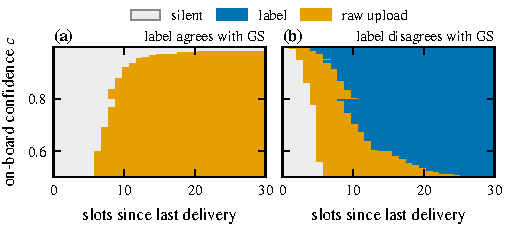
\includegraphics[width=\columnwidth]{figures/regions.pdf}
\caption{Decisions of~\eqref{eq:rule} versus the slots since the last delivery and the confidence, with parameters estimated on Sen1Floods11: GS reports ``not flooded'' with $5\%$ initial doubt, UAV $1.2$\,km from the GS ($q_1\approx1$, $q_2=0.78$, $E_1=20$\,mJ, $E_2=190$\,mJ), $\lambda/V=2$\,J$^{-1}$, $\nu=0.25$. The steps at $c=0.8$ and $c=0.9$ come from the binned estimate of $\ee_{\rm g}(c)$.}
\label{fig:regions}
\end{figure}

Fig.~\ref{fig:regions} shows the decision regions of~\eqref{eq:rule} for the scenario of the example, as a function of the slots since the last delivery and of the confidence. It uses the confidence-dependent $\ee_{\rm g}(c)$ estimated from our data, which Proposition~\ref{prop:threshold} does not cover; the order silent, raw, label still holds. When the label disagrees with the GS, the confidence needed to send it falls as the GS status ages, because the prior probability that the GS is wrong grows. When the label agrees with the GS but is unsure, the UAV uploads the frame once the status is old enough, which amounts to asking the GS to verify its status.
